% Source: report/sections/06_failure_analysis.md (owner: Manoj, #6).
\section{Failure analysis: small and flat polyps}
\label{sec:failure}
A mean Dice of 0.85 or 0.92 hides where a model fails. Clinically, the polyps that doctors miss most often are the
\textbf{small} and the \textbf{flat (sessile)} ones (\cref{sec:intro}). In this section we split the 120 test images into groups
and check whether the models fail on the same polyps that doctors do.

\subsection{How the groups are defined}
\label{sec:groups-def}
\begin{itemize}
  \item \textbf{Size:} the polyp's share of the image, measured on the original-resolution mask.
        Small $<$ 5\%, medium 5--20\%, large $>$ 20\%.
  \item \textbf{Morphology:} a test image is \textbf{sessile/flat} if it is listed in Kvasir-Sessile~\cite{jha2021sessile}, a set of
        196 Kvasir-SEG polyps that experts labelled sessile and smaller than 10\,mm. This is a real expert label.
  \item \textbf{Contrast:} the colour difference ($\Delta E$ in CIELAB colour space) between the polyp and a ring of tissue
        12 pixels wide around it, measured on the $352\times352$ image. The test set is split into thirds: low, mid and high contrast. A low value means the
        polyp blends into the colon wall. This is only a \textbf{stand-in} for ``hard to see'', computed by us, not an expert label.
  \item \textbf{Miss rate:} the share of images with Dice $<$ 0.5, meaning the polyp was essentially not found. A missed polyp
        is clinically worse than a slightly wrong outline, so we report it next to the mean Dice.
\end{itemize}
Some groups are small ($n = 27$ small polyps, 31 sessile polyps), so a single image moves a group's mean noticeably.
We therefore give $n$ for every group and treat differences of a few hundredths with caution.

\subsection{Results by group}
\label{sec:groups}

\begin{table*}[t]
  \centering
  \small
  \begin{adjustbox}{max width=\textwidth}
  \begin{tabular}{@{}lcccccc@{}}
    \toprule
    Group & $n$ & U-Net (scratch) & ResNet-34 & MobileNetV2 & Attention U-Net & SegFormer \\
    \midrule
    Small ($<$ 5\%)   & 27 & 0.713 (18.5\%) & 0.851 (7.4\%) & 0.812 (11.1\%) & 0.730 (22.2\%) & 0.862 (7.4\%) \\
    Medium (5--20\%)  & 58 & 0.900 (0.0\%)  & 0.934 (0.0\%) & 0.934 (1.7\%)  & 0.906 (0.0\%)  & 0.948 (0.0\%) \\
    Large ($>$ 20\%)  & 35 & 0.876 (0.0\%)  & 0.891 (5.7\%) & 0.890 (5.7\%)  & 0.862 (0.0\%)  & 0.908 (2.9\%) \\
    \midrule
    Sessile/flat      & 31 & 0.734 (12.9\%) & 0.850 (6.5\%) & 0.826 (9.7\%)  & 0.758 (16.1\%) & 0.867 (6.5\%) \\
    Other             & 89 & 0.892 (1.1\%)  & 0.922 (2.2\%) & 0.917 (3.4\%)  & 0.887 (1.1\%)  & 0.934 (1.1\%) \\
    \midrule
    Low contrast      & 40 & 0.836 (5.0\%)  & 0.896 (2.5\%) & 0.883 (7.5\%)  & 0.861 (2.5\%)  & 0.907 (2.5\%) \\
    Mid contrast      & 40 & 0.825 (7.5\%)  & 0.869 (7.5\%) & 0.865 (7.5\%)  & 0.823 (10.0\%) & 0.898 (5.0\%) \\
    High contrast     & 40 & 0.892 (0.0\%)  & 0.943 (0.0\%) & 0.933 (0.0\%)  & 0.876 (2.5\%)  & 0.946 (0.0\%) \\
    \bottomrule
  \end{tabular}
  \end{adjustbox}
  \caption{Mean test Dice (miss rate) per group.}
  \label{tab:groups}
\end{table*}

\Cref{tab:groups} gives the mean Dice and miss rate per group. \Cref{fig:failure} shows the same means as bar charts, and
\cref{fig:dicesize} plots the Dice of every test image against its polyp size.

\begin{figure*}[t]
  \centering
  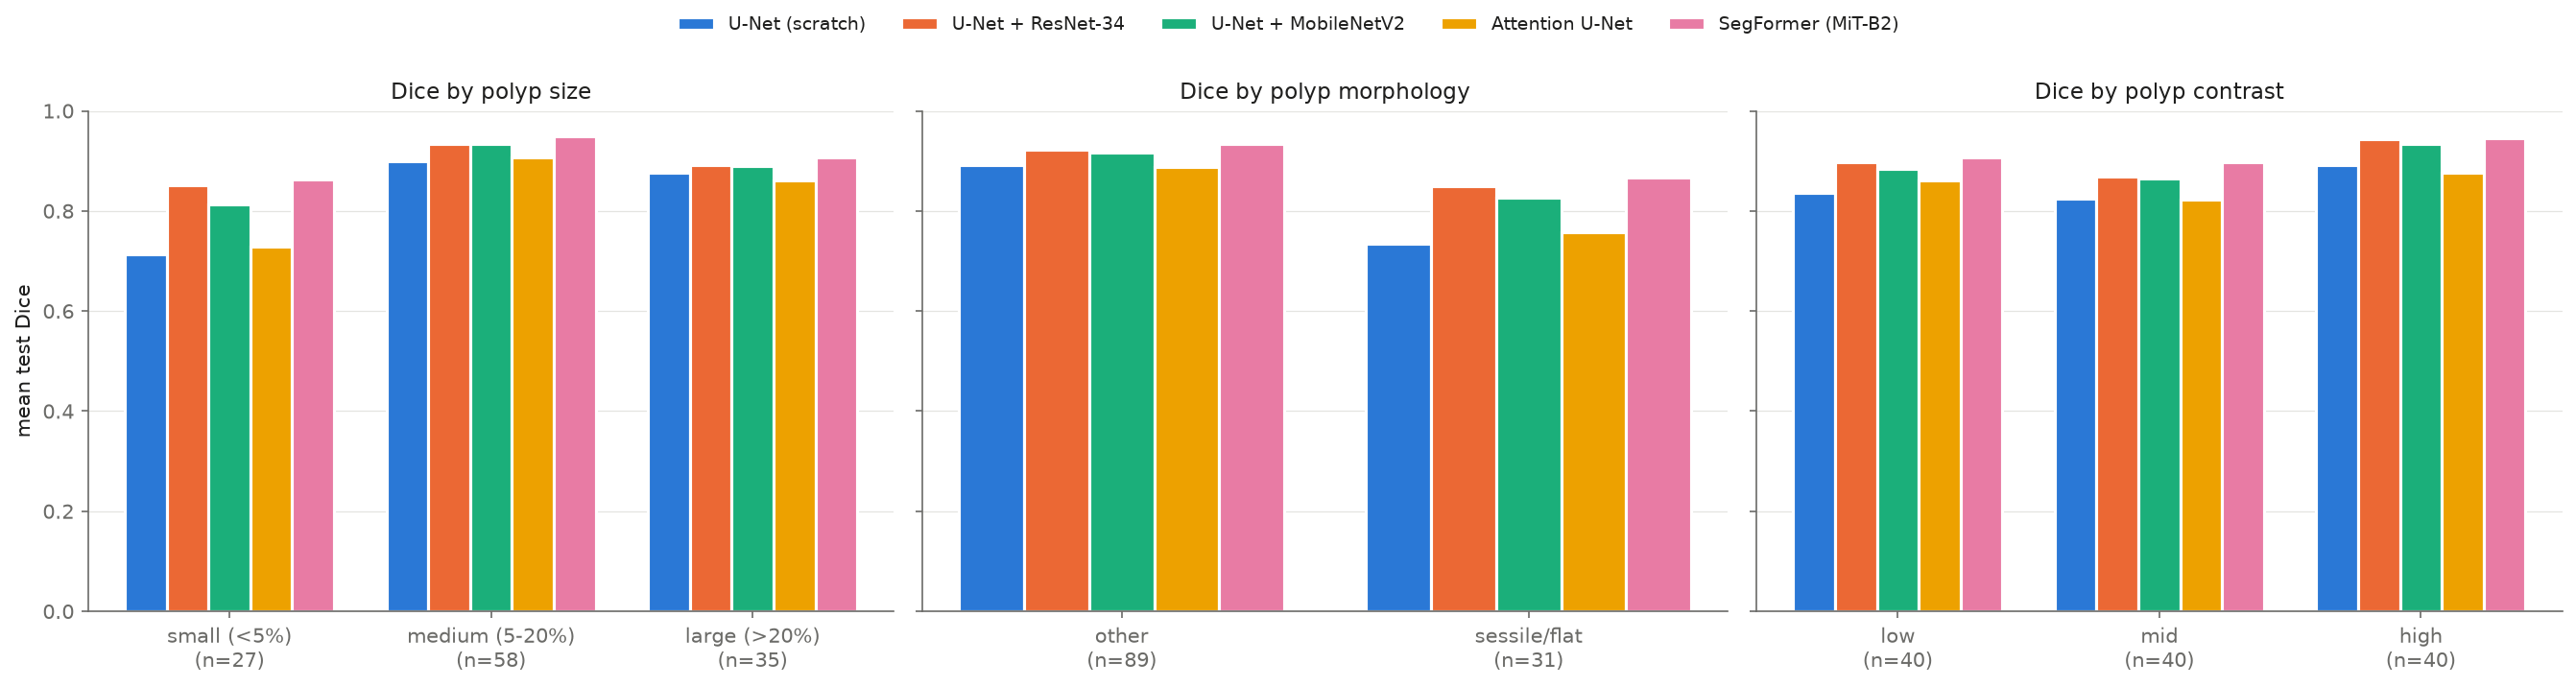
\includegraphics[width=\textwidth]{failure_analysis.png}
  \caption{Mean test Dice per group: polyp size, morphology (Kvasir-Sessile) and contrast.}
  \label{fig:failure}
\end{figure*}

\begin{figure*}[t]
  \centering
  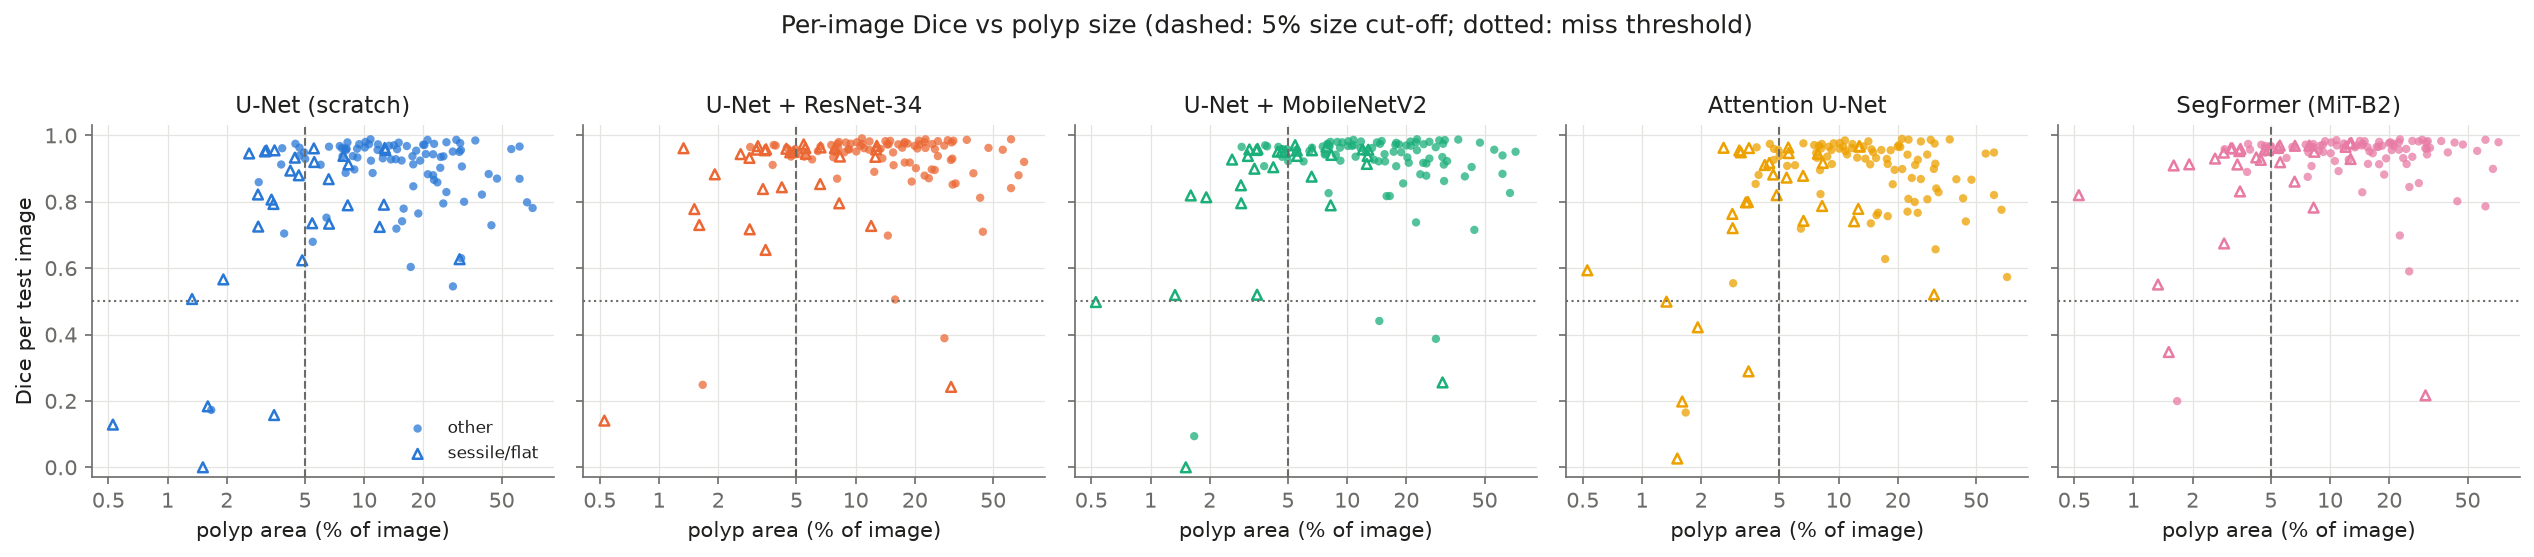
\includegraphics[width=\textwidth]{dice_vs_size.png}
  \caption{Dice of every test image against polyp size (log scale), one panel per model. Triangles: sessile polyps; dashed line: 5\% size cut-off; dotted line: miss threshold (Dice 0.5).}
  \label{fig:dicesize}
\end{figure*}

\paragraph{Small polyps are the main weakness.} The baseline scores 0.713 on small polyps against 0.900 on medium ones,
and it misses 5 of the 27 small polyps (18.5\%). It misses no medium or large polyp at all: all five complete
misses in the test set are small polyps. The Attention U-Net behaves the same way (0.730 on small polyps, 6 of
27 missed, again all of its misses are small polyps), so the attention gates do not help where help is needed
most. \textbf{Pretrained encoders narrow the gap most.} ResNet-34 raises the Dice on small polyps by 0.138
($0.713 \rightarrow 0.851$) and SegFormer by 0.149 ($\rightarrow 0.862$), far more than their gains on medium polyps (+0.034 and
+0.048). Both miss only 2 of the 27 small polyps (7.4\%); MobileNetV2 is in between (0.812, 3 missed). The
improvement from a pretrained encoder is therefore largest exactly on the hard cases, not only on polyps that
were already easy.

\paragraph{Flat polyps are almost as hard.} For the baseline, sessile polyps score 0.734 against 0.892 for the others,
with a miss rate of 12.9\% against 1.1\%. The Attention U-Net is similar (0.758, 16.1\% missed). ResNet-34 and
SegFormer halve the miss rate on sessile polyps, to 6.5\% (2 of 31), with Dice 0.850 and 0.867; MobileNetV2
lowers it less, to 9.7\% (Dice 0.826). A gap to the other polyps remains for every model
(SegFormer 0.867 against 0.934).

\paragraph{Small and flat overlap.} The two groups are largely the same polyps: 18 of the 27 small polyps are sessile,
because Kvasir-Sessile only contains polyps under 10\,mm. \Cref{tab:size-morph} separates the two factors.

\begin{table*}[t]
  \centering
  \small
  \begin{adjustbox}{max width=\textwidth}
  \begin{tabular}{@{}lcccccc@{}}
    \toprule
    Group & $n$ & U-Net (scratch) & ResNet-34 & MobileNetV2 & Attention U-Net & SegFormer \\
    \midrule
    Other, not small   & 80 & 0.899 (0.0\%)  & 0.927 (1.2\%)  & 0.924 (2.5\%)  & 0.896 (0.0\%)  & 0.942 (0.0\%) \\
    Other, small       & 9  & 0.826 (11.1\%) & 0.874 (11.1\%) & 0.858 (11.1\%) & 0.804 (11.1\%) & 0.870 (11.1\%) \\
    Sessile, not small & 13 & 0.840 (0.0\%)  & 0.863 (7.7\%)  & 0.878 (7.7\%)  & 0.848 (0.0\%)  & 0.880 (7.7\%) \\
    Sessile, small     & 18 & 0.657 (22.2\%) & 0.840 (5.6\%)  & 0.789 (11.1\%) & 0.693 (27.8\%) & 0.858 (5.6\%) \\
    \bottomrule
  \end{tabular}
  \end{adjustbox}
  \caption{Mean test Dice (miss rate) by size and morphology together.}
  \label{tab:size-morph}
\end{table*}

For the two CNNs trained from scratch, both factors lower the Dice on their own, and polyps that are both small
and flat are by far the hardest: the baseline misses 4 of these 18 polyps and the Attention U-Net 5. The
pretrained encoders shrink this weakness: MobileNetV2 misses 2 of the 18, and ResNet-34 and SegFormer only 1
each. For SegFormer (0.858) and ResNet-34 (0.840), the Dice on small sessile polyps is close to their Dice on the
other groups; MobileNetV2 still lags (0.789). With only 9 and 13 images in two of the cells, where one image
changes the miss rate by 8--11 points, this split is indicative only.

\paragraph{Contrast matters less than size.} All five models score lower on low- and mid-contrast polyps than on
high-contrast ones: for the baseline about 0.83 against 0.89, for ResNet-34 0.896 and 0.869 against 0.943, and
for SegFormer 0.907 and 0.898 against 0.946. The effect is smaller than for size, and low and mid contrast are
not clearly different. Sessile polyps do have lower contrast (median $\Delta E$ 19.6 against 42.0), which fits the
clinical picture of flat lesions that blend into the wall.

\paragraph{A new failure mode: large polyps.} The models trained from scratch miss no polyp larger than 5\% of the image,
but the three pretrained models each miss one or two large ones. Two large polyps (28\% and 31\% of the image, the
second one sessile) are missed by both ResNet-34 and MobileNetV2, and the second one also by SegFormer, while
both scratch models find them. Pretraining therefore trades many misses on small polyps for a few misses on
large ones. Both images show the same pattern: the polyp has a raised, dome-shaped part and a large flat part
around it, and the pretrained models outline only the dome. On the sessile one (\texttt{ck2bxw\dots}, row 2 of \cref{fig:worst})
all three pretrained models mark only a small round nodule at the lower edge of a lesion that covers almost a
third of the image. The scratch U-Net covers more of the flat area, though with a patchy, low-confidence mask.
The pretrained encoders seem to have learned a strong idea of a polyp as a compact, raised blob, which helps them
find small polyps but makes them overlook wide, flat lesions.

\subsection{Worst cases}
\label{sec:worst}
\Cref{fig:worst} shows the eight test images on which the best model, SegFormer, scored
lowest, with the ground truth in green and the prediction in red. Likely reasons:

\begin{figure}[!t]
  \centering
  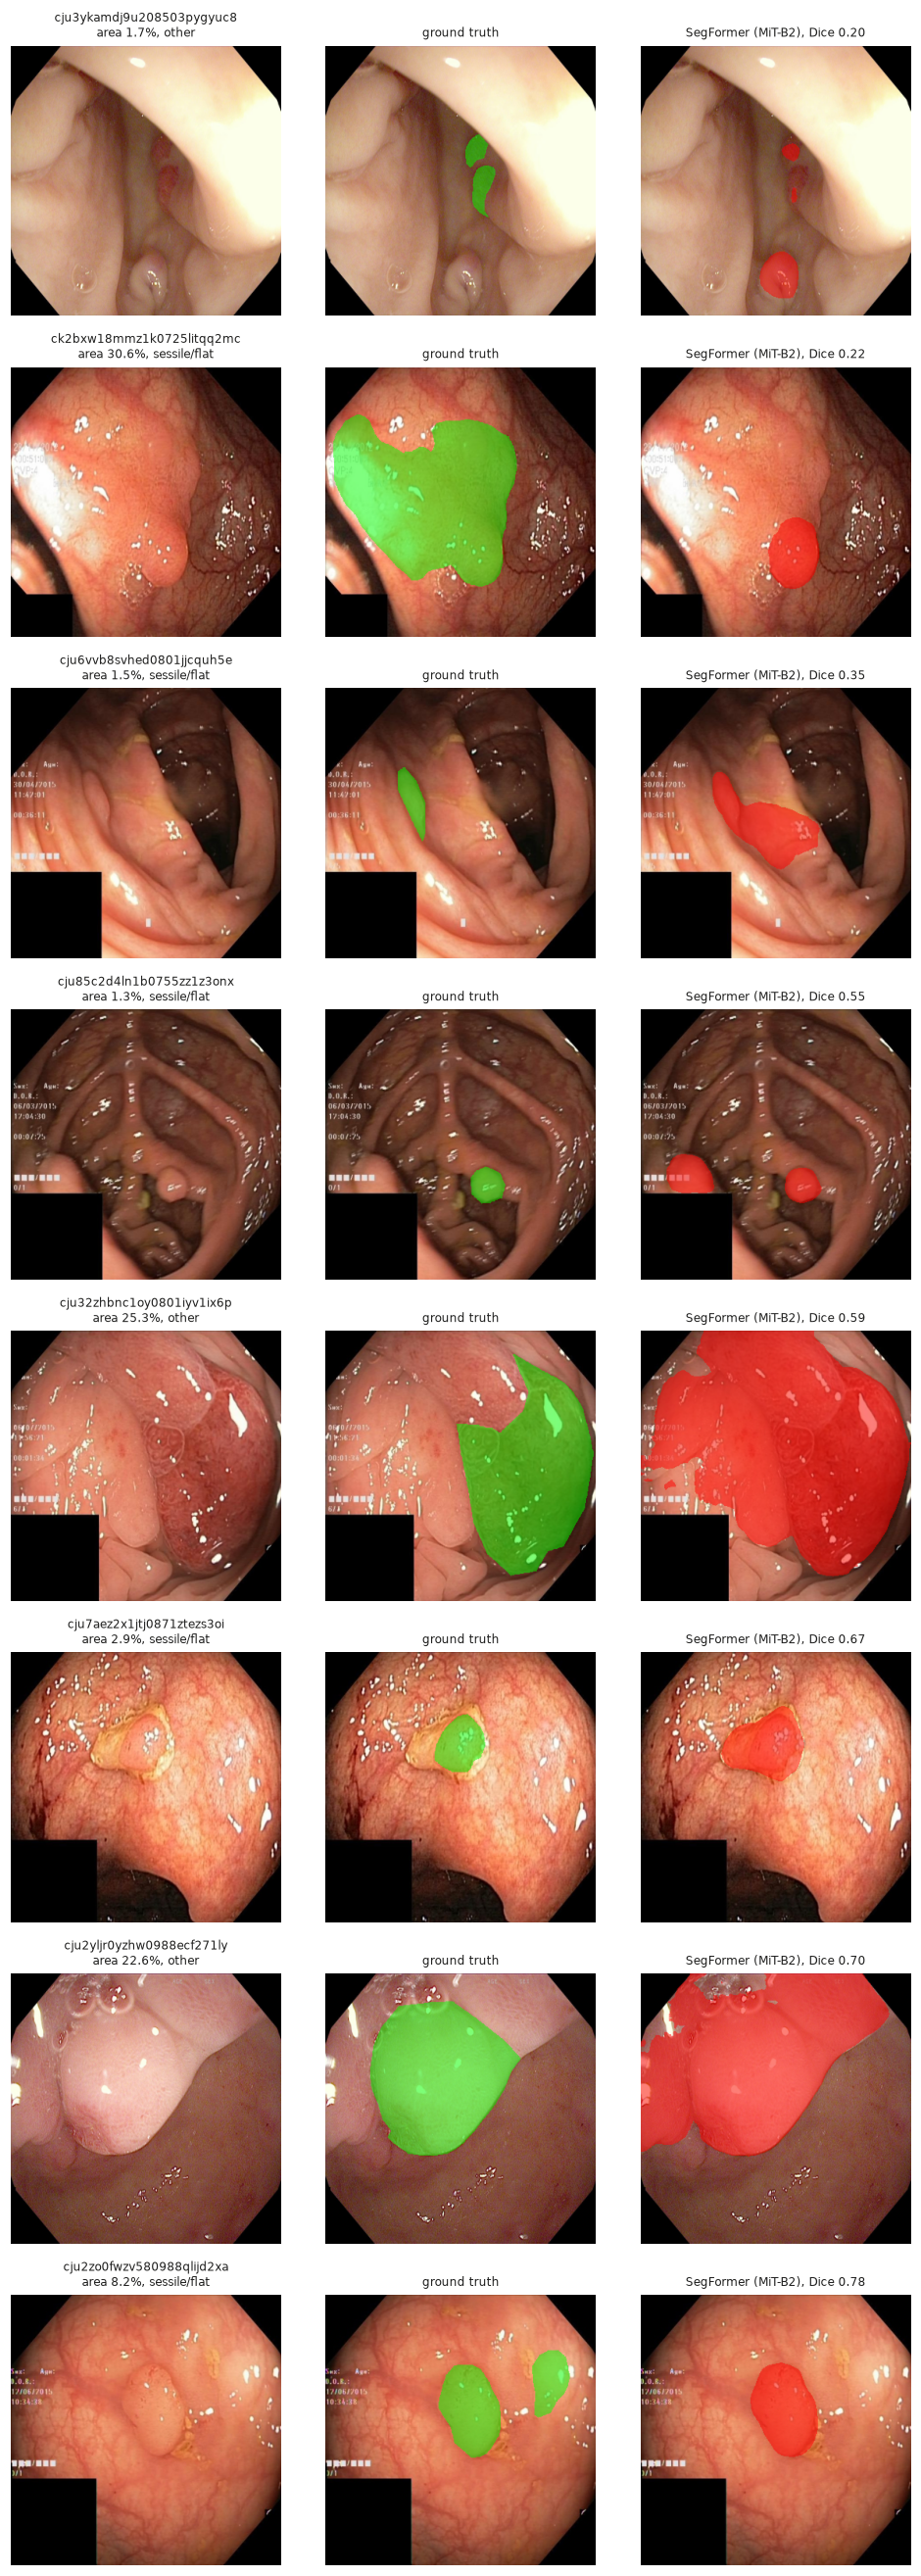
\includegraphics[height=0.72\textheight,keepaspectratio]{worst_cases.png}
  \caption{The eight test images on which SegFormer scored lowest: ground truth in green, prediction in red.}
  \label{fig:worst}
\end{figure}

\begin{enumerate}
  \item \texttt{cju3ykamdj\dots} (1.7\% of the image, Dice 0.20): a tiny reddish polyp in a fold next to an over-exposed bright
        fold. SegFormer marks only a sliver of it and marks a round bump of normal tissue below it instead.
  \item \texttt{ck2bxw18mm\dots} (30.6\%, sessile, Dice 0.22): a large flat lesion that blends into the wall, with glare at the
        upper left. SegFormer finds only the raised nodule at its lower edge (see \cref{sec:groups}).
  \item \texttt{cju6vvb8sv\dots} (1.5\%, sessile, Dice 0.35): a small flat polyp on a fold. The prediction covers it but spreads
        along the fold onto neighbouring tissue, so most of the predicted area is wrong.
  \item \texttt{cju85c2d4l\dots} (1.3\%, sessile, Dice 0.55): the small polyp is found correctly, but a second round structure at
        the left edge of the image, next to the black overlay box, is also marked as a polyp.
  \item \texttt{cju32zhbnc\dots} (25.3\%, Dice 0.59): the polyp is found, but the prediction also covers the large neighbouring fold
        on its left, which has a similar colour and texture.
  \item \texttt{cju7aez2x1\dots} (2.9\%, sessile, Dice 0.67): the polyp sits inside a yellowish rim. The ground truth covers only
        the central part and the prediction includes the rim, where the true border is ambiguous.
  \item \texttt{cju2yljr0y\dots} (22.6\%, Dice 0.70): a pale, glossy polyp with strong glare. The prediction extends onto the fold
        above and to the left of it.
  \item \texttt{cju2zo0fwz\dots} (8.2\%, sessile, Dice 0.78): the image contains two polyps. SegFormer outlines the larger one
        well but misses the second.
\end{enumerate}
Four of the eight are small polyps and five are sessile, so the groups of \cref{sec:groups} are again
over-represented. Only three of the eight (images 1--3) are misses with Dice below 0.5. In the other five,
SegFormer finds the polyp but gets its extent wrong: four times it spreads onto a neighbouring fold or rim, and
once it misses a second polyp. Its remaining errors are therefore mostly about \textbf{where the polyp ends} rather than
\textbf{whether there is a polyp}, the opposite of the scratch models, whose failures are mostly missed small polyps.

\subsection{What this means}
\label{sec:failure-meaning}
SegFormer and U-Net + ResNet-34 are the most reliable models on the polyps that matter most clinically. Each
misses only 2 of the 27 small polyps and 1 of the 18 small sessile polyps, against 5 and 4 for the baseline, and
they miss 3 and 4 of the 120 test polyps overall, against 5 for the baseline. Their misses are not limited to
small polyps, as the scratch models' are: each misses at least one large polyp, so they fail less often but not
in a fully predictable way. Small and flat polyps remain the weakest groups for every model, so they still need
the doctor's full attention.
